\documentclass[border=2mm,
               tikz,
               preview]{standalone}
\usetikzlibrary{positioning,chains}
\usepackage{xcolor}
\definecolor{titlebg}{HTML}{FFC000}
\definecolor{labelbg}{HTML}{9DC3E6}

\begin{document}

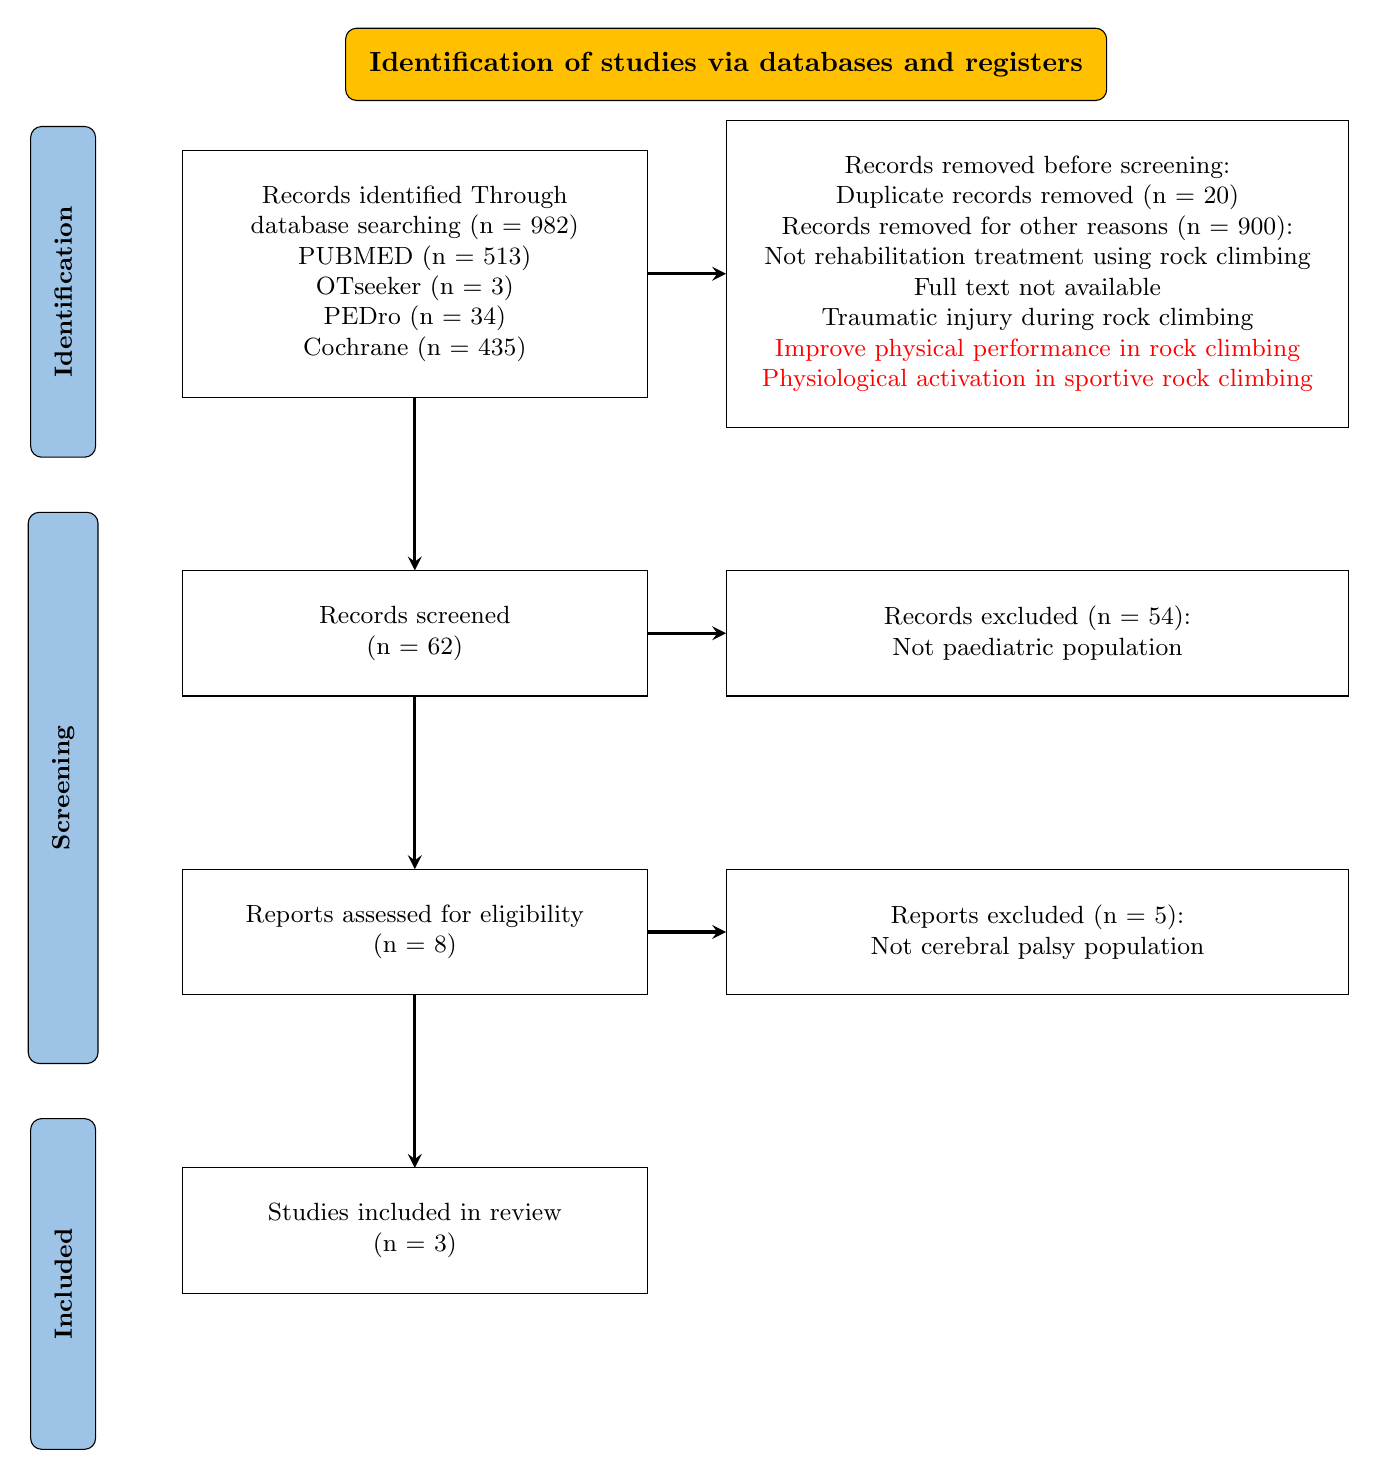
\begin{tikzpicture}[
    node distance=22mm and 10mm,
    start chain=going below,
 mynode/.style = {
        draw, rectangle, align=center, text width=5cm,
        font=\small, inner sep=3ex, outer sep=0pt,
        on chain},
 mynodeR/.style = {
        draw, rectangle, align=center, text width=7cm,
        font=\small, inner sep=3ex, outer sep=0pt,
        on chain},
title/.style = {
        draw, rectangle, align=center, rounded corners,
        font=\small\bfseries, inner sep=2ex, outer sep=0pt,
        fill=titlebg,
        on chain},
mylabel/.style = {
        draw, rectangle, align=center, rounded corners, 
        font=\small\bfseries, inner sep=2ex, outer sep=0pt,
        fill=labelbg, minimum height=42mm,
        on chain},
mylabellong/.style = {
        draw, rectangle, align=center, rounded corners, 
        font=\small\bfseries, inner sep=2ex, outer sep=0pt,
        fill=labelbg, minimum height=70mm,
        on chain},
every join/.style = arrow,
     arrow/.style = {very thick,-stealth}
                    ] 
\coordinate (tc);
% the title
\node[title,above=of tc,font=\bfseries] {Identification of studies via databases and registers};

% the nodes at the top
\node (n1a) [mynode, left=of tc]    {Records identified Through database searching
(n~=~982)  \\
PUBMED (n~=~513)\\
OTseeker (n~=~3) \\
PEDro (n~=~34) \\
Cochrane (n~=~435)\\
};
\node (n1b) [mynodeR,right=of n1a]    {Records removed before screening:\\
Duplicate records removed (n~=~20)\\
Records removed for other reasons (n~=~900): \\
Not rehabilitation treatment using rock climbing\\
Full text not available\\
Traumatic injury during rock climbing\\
\textcolor{red}{Improve physical performance in rock climbing}\\
\textcolor{red}{Physiological activation in sportive rock climbing}};
    % the chain in the center
\node (n2)  [mynode,below=of n1a]   {Records screened\\
(n~=~62)};
\node (n3)  [mynode,join,below=of n2]   {Reports assessed for eligibility\\
(n~=~8)};
\node (n4)  [mynode,join]   {Studies included in review\\
(n~=~3)};
% the branches to the right
\node (n2r) [mynodeR,right=of n2]    {Records excluded (n~=~54):\\
Not paediatric population};
\node (n3r) [mynodeR,right=of n3]    {Reports excluded (n~=~5):\\
Not cerebral palsy population};
% lines not included in join                                        
\draw[arrow] (n1a) -- (n2);
\draw[arrow] (n1a) -- (n1b);
\draw[arrow] (n2) -- (n2r);
\draw[arrow] (n3) -- (n3r);
% the labels on the left
    \begin{scope}[node distance=7mm]
\node[mylabel,below left=-3mm and 11mm of n1a.north west]
                {\rotatebox{90}{Identification}};
\node[mylabellong]  {\rotatebox{90}{Screening}};
\node[mylabel]  {\rotatebox{90}{Included}};
    \end{scope}
\end{tikzpicture}
\end{document}